\documentclass{article}

\usepackage{tikz}
\usepackage{pgfplots}
\pgfplotsset{compat=newest}
\begin{document}
\begin{figure}[h]
  \begin{center}

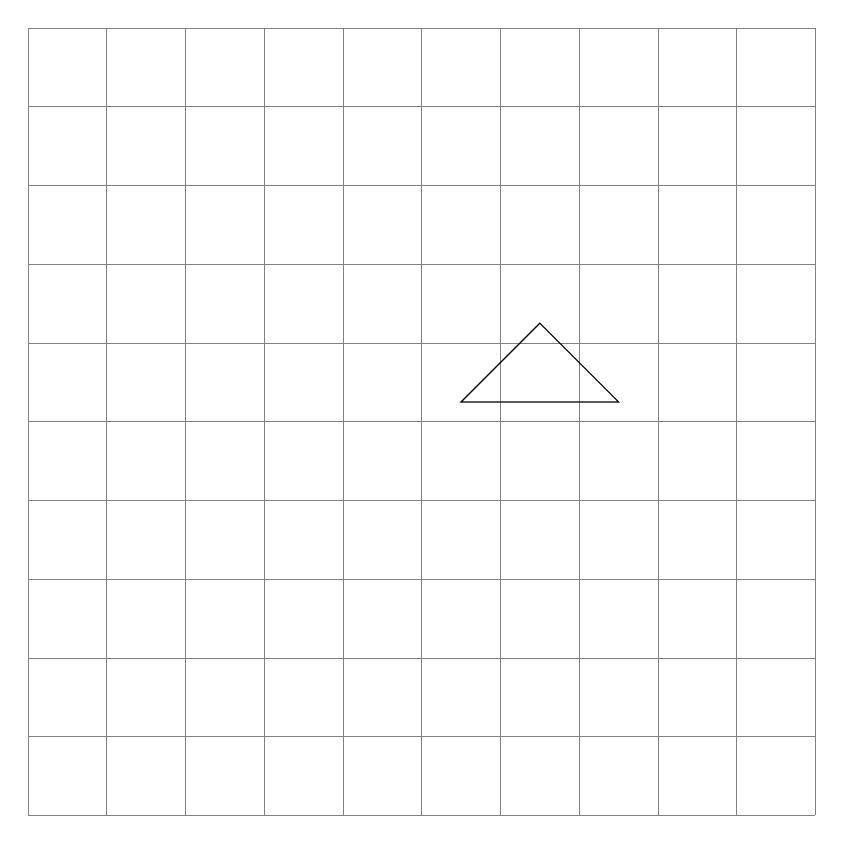
\begin{tikzpicture}

  \draw[very thin, gray] (-5, -5) grid (5, 5);

  %\draw (0,0) node[below] {$(0, 0)$};
  
  % \draw (0, 0) % (0, 0)
  %  node[below] {$(0, 0)$} 
  % -- ++(1,1) % relatively (1, 1)
  %  node[above] {$(1, 1)$} 
  % -- ++(1,-1) % (2, 0)
  %  node[below] {$(2, 0)$} -- cycle;

  \draw (0.5, 0.25) 
  -- ++(1, 1)
  -- ++(1, -1) -- cycle;

\end{tikzpicture}
\end{center}
  \caption{Absurd Thing}
\end{figure}


\end{document}